\chapter{Hybridní hry}
Hybridní hry kombinují jak prvky fyzické, tak digitální. Jedná se o~hry, které mají jakékoliv napojení na technologii, ať už je to elektronické bankovnictví ve hře \textit{Monopoly Super Electronic Banking} či mobilní aplikace \textit{Pokémon GO}, která uživatele pomocí map navádí k~navštívení památek a~zajímavých míst. Podobná spojení vyústí ve zcela nové herní zážitky, které si hráči mohou vyzkoušet. \cite{hybrid_board_games_design}

\section{Vývoj hybridních her}
První hybridní hry se začaly formovat již na začátku 20. století, kdy se začaly objevovat první hry s~elektronickými prvky. Tyto hry byly většinou jednoduché elektrické obvody, které hráč propojoval pro různé efekty. V~průběhu času se tyto hry stávaly složitějšími a~začaly se objevovat takové, které využívaly počítačové technologie. Hybridní hry mohou být kategorizovány do několika skupin, které se liší podle toho, jakým způsobem technologie využívají. \cite{history_of_hybrid_games}

\subsection{Stolní hry s~vlastním zařízením}
Mezi takovéto hry patří již výše zmíněné \textit{Monopoly Super Electronic Banking}, které obsahují elektronické bankovnictví, nebo známá hra \textit{Operation}, ve které se hráči nesmí dotknout kovových částí na hrací desce, jinak se rozezní siréna. 

Tato kategorie hybridních her je rozhodně nejstarší. První hrou využívající elektrického proudu, a~tudíž zařazenou do hybridních her, je hra \textit{Electra} (původním názvem \textit{Lichtra}), kterou můžeme vidět na Obrázku \ref{fig:electra}. Jedná se o~jednoduchou kvízovou hru, která vyšla už v~roce 1910 v~Německu a~byla vytvořena společností \textit{Sala Games}. Hra obsahovala jednoduchý elektrický obvod, který se uzavřel, pokud hráč odpověděl správně. Po ní následovala dlouhá éra her, jejichž elektronika také spočívala pouze v~propojení jednoho či několika málo obvodů. \cite{history_of_hybrid_games, boardgames_with_apps}

\begin{figure}[H]
    \centering
    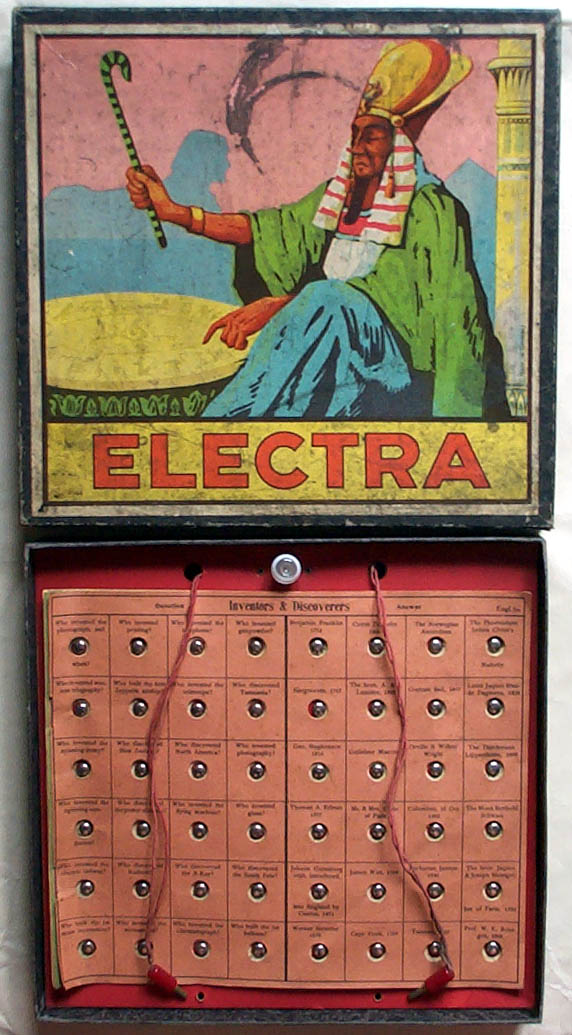
\includegraphics[width=0.3\textwidth]{resources/figures/electra.jpg}
    \caption{Hra \textit{Electra}, první hybridní hra \cite{history_of_hybrid_games}}
    \label{fig:electra}
\end{figure}

Další zmínku ve vývoji her v~této kategorii si zasloužila hra \textit{Voice of the Mummy}, která vyšla v~roce 1971. Ta měla v~herním plánu zabudovaný přehrávač, který měl simulovat hlas mumie, která při přechodu přes určitá herní pole hráčům určovala další postup. \cite{voice_of_the_mummy}

První hrou, která ve svém designu používala počítačové zařízení, byla francouzská hra \textit{Simulateur JR10}, která vyšla v~roce 1972. Jednalo se o~bitevní hru, ve které hráči ovládali různé bojové jednotky. Při střetu se do počítače vložil děrný štítek s~odpovídajícími jednotkami a~počítač podle naprogramovaných kritérií náhodně určil výsledek střetu. \cite{simulateur_jr10}

\subsection{Stolní hry s~vlastní aplikací}
V~roce 1972 vyšla herní konzole \textit{Magnavox Odyssey}, která je uznávaná jako první domácí herní konzole na světě. Zároveň s~ní vyšlo i~několik her, které kombinovaly fyzickou hrací desku s~počítačovým programem. Celé UI této konzole zahrnovalo pouze několik svítících bodů na obrazovce, proto byl ke každé hře přiložen lehce průsvitný plán s~potiskem, který se na obrazovku přichytil. Součástí většiny her byly i~fyzické komponenty, které měly hráčům sloužit k~přirozenějšímu pozvolnému přechodu ze stolních her na hry digitální. \cite{magnavox_odyssey} Jednou z~her vytvořenou pro tuto konzoli byla hra \textit{Invasion}, jejíž fyzická složka zahrnovala kostky, sadu karet, sadu tokenů a~hrací desku. Samotný program byl pak určen k~soubojům mezi hráči. Tyto komponenty můžeme vidět na Obrázku \ref{fig:invasion} \cite{invasion,invasion_gameplay}

\begin{figure}[H]
    \centering
    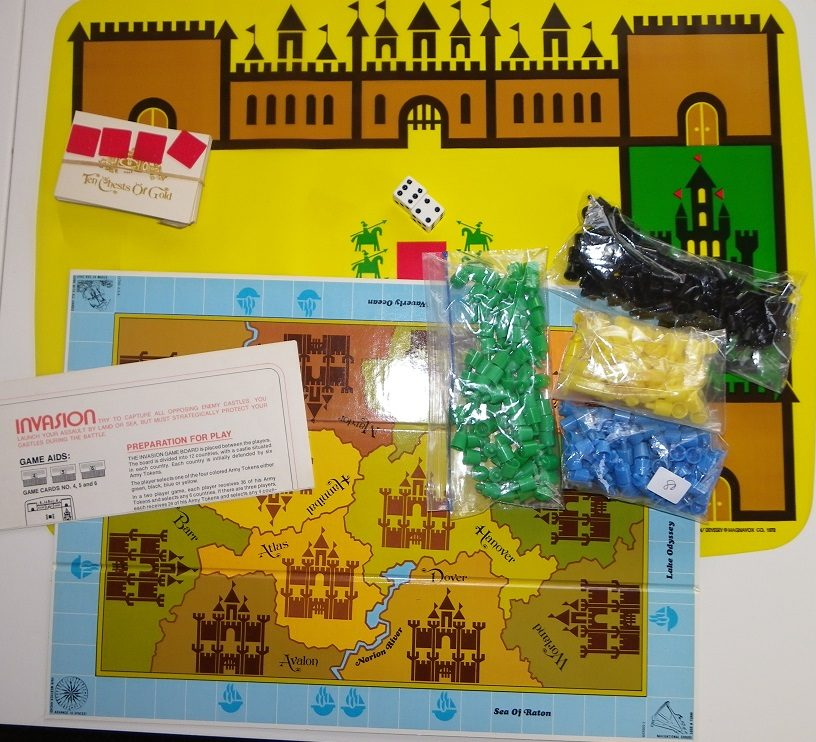
\includegraphics[width=0.45\textwidth]{resources/figures/invasion.jpg}
    \caption{Fyzické komponenty a~nalepovací plán hry \textit{Invasion} \cite{invasion}}
    \label{fig:invasion}
\end{figure}

V~roce 1983 vyšlo hned několik her, které kombinovaly fyzickou hrací desku s~digitálním prostředím. Jednou z~nich byla společností \textit{Epyx} vydaná hra \textit{Oil Barons}. Jednalo se o~počítačovou hru, která byla určena pro zařízení \textit{DOS}, \textit{Apple II} a~\textit{Commodore 64}. Její součástí byla fyzická hrací deska a~několik herních tokenů. Samotný program měl za úkol simulovat náhodné výsledky a~udržovat stav hry. UI této hry bylo jednoduché a~odpovídalo své době, jak lze vidět na Obrázku \ref{fig:oil_barons}. \cite{oil_barons}

\begin{figure}[H]
    \centering
    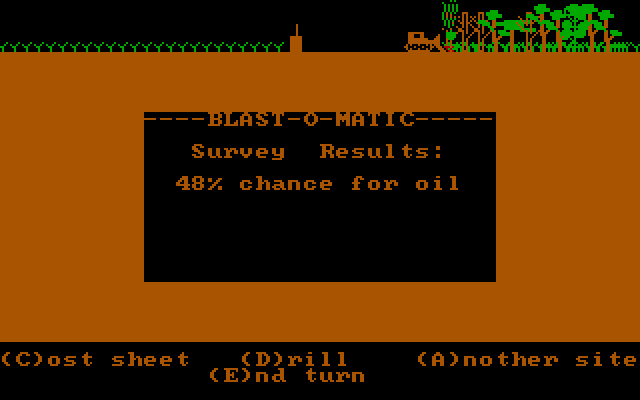
\includegraphics[width=0.45\textwidth]{resources/figures/oil_barons.png}
    \caption{Příklad GUI hry \textit{Oil Barons} \cite{oil_barons}}
    \label{fig:oil_barons}
\end{figure}

Další významný vývoj této kategorie hybridních her se ubíral nejčastěji k~mobilním aplikacím a~takzvaným companion apps (podpůrným aplikacím). Tyto aplikace slouží k~různým účelům, jako je například výběr či správa herních prvků nebo vyprávění příběhu. Většina těchto aplikací je oficiální součástí dané hry a~bez jejího použití není možné ji odehrát. Mezi ně patří například hra \textit{Na vlnách neznáma} (původním názvem \textit{Forgotten Waters}), která využívá aplikaci k~vyprávění příběhu, správě nepřátel a~k~výběru dějové linky.

\subsection{Hry s~rozšířenou realitou}
Nejmladší kategorií hybridních her jsou hry s~rozšířenou realitou (augmented reality, neboli AR). Tyto hry využívají technologie, které umožňují hráčům interagovat s~digitálními prvky ve skutečném světě. První takovou hrou byla \textit{AR Quake}, která byla vytvořena v~roce 2000. Aby si ji hráč mohl vyzkoušet, musel mít nasazený speciální batoh s~počítačem, který pomocí gyroskopů určoval jeho polohu a~promítal obraz digitálního světa přes speciální brýle. Hra byla vytvořena jako experiment, který měl ukázat možnosti AR technologií. \cite{ar_history}

Největší rozvoj v~popularitě AR her nastal až s~vydáním aplikace \textit{Pokémon GO} v~roce 2016. Tato hra využívala GPS a~kameru mobilního telefonu k~tomu, aby hráči ve skutečném světě mohli hledat a~chytat virtuální postavičky. Hra byla velice populární a~stala se tak první AR hrou, která se dostala do povědomí široké veřejnosti.

\section{Vybrané hybridní hry}
Následující hry jsem vybral jako příklady a~inspiraci pro tuto práci. Jedná se o~stolní hry, které nějakým způsobem využívají právě internetových aplikací pro umocnění herního zážitku, organizaci hry či správu herních mechanismů.

\subsection{Na vlnách neznáma}
První z~těchto her je \textit{Na vlnách neznáma}, vydaná v~roce 2020 společností \textit{Plaid Hat Games}. Jedná se o~výpravnou RPG hru, ve které se hráči ujímají rolí pirátů a~společně čelí dobrodružstvím a~nástrahám, jež rozmanitý příběh této hry nabízí. Hra samotná využívá oficiální internetovou aplikaci \cite{forgotten_waters_app}, která slouží k~vyprávění herního děje pomocí namluvených scén a~k~zaznamenávání hráčských rozhodnutí, na kterých závisí dynamický rozvoj příběhu této hry. Aplikace dále udává životy a~statistiky nepřátel, slouží k~výběru kampaně (dějové linky) a~v~neposlední řadě přispívá k~zážitku hráčů pomocí namluvených scén.

Fyzické komponenty hry obsahují herní plán s~hexagonálními políčky a~s~tokeny lokací, které si hráči rozestaví podle pokynů aplikace. Dále obsahuje kartonové figurky, osobní deníky postav, knihu lokací, balíček karet a~sadu kostek. Kartonové figurky s~potiskem v~kombinaci s~osobními deníky, do kterých si hráči zapisují informace, představují postavy. Zároveň se ve hře nachází několik ukazatelů a~počítadel, jež se využívají v~různých aspektech hry. V~knize lokací lze najít popisy míst, které mohou hráči ve hře navštívit, a~zároveň možnosti, jež se jim v~těchto lokacích nabízejí. Karty v~balíčku představují poklady a~úryvky příběhu. Oba tyto druhy přináší hráči buďto pozitivní nebo negativní efekty, které ovlivňují jeho postavu. Sada kostek se využívá k~určování výsledků různých akcí, jež hráči mohou provést.

\subsection{Gloomhaven}
Druhou hrou, kterou bych chtěl uvést, je \textit{Gloomhaven}. Tato hra byla vydána v~roce 2017 společností \textit{Cephalofair Games}. Jde o~kooperativní fantasy hru, ve které se hráči vcítí do role dobrodruhů, jenž se snaží přežít v~nehostinném světě, plnit různé úkoly a~odkrývat příběh, který před nimi leží. Hra je ve stylu dungeon crawl, což znamená, že hlavní náplní hry je postup z~lokace do lokace, kde hráče čekají úkoly a~boj s~nepřáteli. Původně je hra koncipována jako čistě stolní hra, ale kvůli velkému množství fyzických komponent (Obrázek \ref{fig:gloomhaven_contents}), které hra obsahuje, začaly vznikat aplikace, jež mají za úkol organizaci hry usnadnit. Jednou z~nich byla aplikace \textit{Gloomhaven Helper} \cite{gloomhaven_helper}, která se na čas stala i~oficiální aplikací pro tuto hru, avšak kvůli licenčním problémům byla zrušena. Po jejím stažení z~trhu vzniklo několik nástupců. Jedním z~nich je \textit{Gloomhaven Secretariat} \cite{gloomhaven_secretariat}, který slouží k~organizaci hry, správě nepřátel i~postav. Také umožňuje hráčům zaznamenávat své postupy v~příběhu, výsledky bitev a~další herní prvky.

\begin{figure}[H]
    \centering
    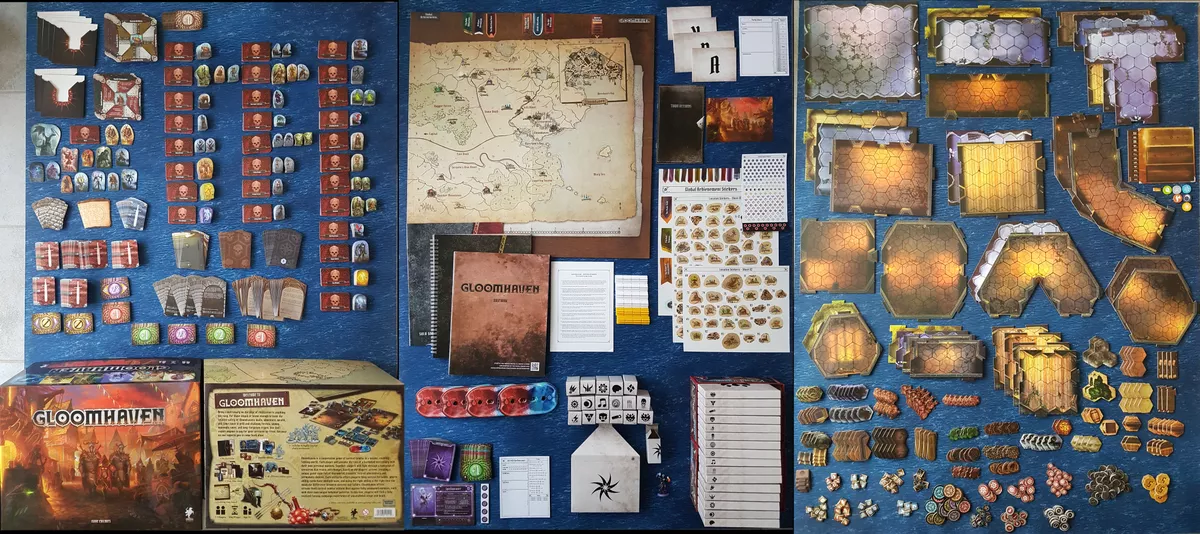
\includegraphics[width=0.9\textwidth]{resources/figures/gloomhaven.png}
    \caption{Fyzické komponenty deskové hry \textit{Gloomhaven} \cite{gloomhaven}}
    \label{fig:gloomhaven_contents}
\end{figure}

Fyzická součást hry obsahuje mapu světa, na kterou hráči postupně přilepují nálepky odemčených lokací a~svých úspěchů. Hra obsahuje díly lokací, což jsou části hrací desky, které lze složit k~sobě. Tyto části jsou potištěny hexagonovou sítí, která slouží jako políčka pro hráčské figurky. Dále se zde nachází kniha lokací, která popisuje příběh a~udává rozložení a~díly potřebné pro složení jednotlivých lokací. Každý typ nepřítele má svou kartu statistik a~vlastní balíček karet, které určují jeho chování a~možné akce. Pro všechny nepřátele existuje jeden společný balíček modifikátorů (karet, které namísto kostek slouží k~vytváření nahodilých výsledků). Podobně má každá postava také svou sadu karet akcí a~velkou kartu statistik, zároveň má však každý hráč vlastní balíček modifikátorů a~počítadlo životů. Figurky postav jsou vyrobeny z~plastu a~jsou velice detailní. Kartonové figurky s~plastovými stojánky představují nepřátele. Dále hra obsahuje velké množství kartiček předmětů, které hráči mohou používat, tokeny peněz, poškození a~efektů.